\begin{center}
\begin{tikzpicture}[x=1cm,y=1cm]
%\pgfresetboundingbox
\draw[use as bounding box, anchor = north west,draw=none] (-5.5,-3.25) rectangle (5.5,3.25);
\clip (-5.5,-3.25) rectangle (5.5,3.25);
\only<1->{\node[anchor =north west] (text) at (-5.25,3.25){\begin{minipage}{10.0cm}
One family of 3D desciptors attempt to copy information used in quantum chemistry codes, e.g. Coulomb Matricies:\\
\scriptsize  Montavon, G. \textit{et al.}. Learning Invariant Representations of Molecules for Atomization Energy Prediction, NIPS 25, 2012 \normalsize
\begin{align*}
M_{I,J} = 
\begin{cases}
0.5Z_{I}^{2.4}& \text{for } I = J \\
\frac{Z_{I}Z_{J}}{|R_I-R_J|}&  \text{for } I \neq J
\end{cases}
\end{align*}		
\end{minipage}};}
\visible<1->{\node[anchor=east] (east) at (3.5,-1.5){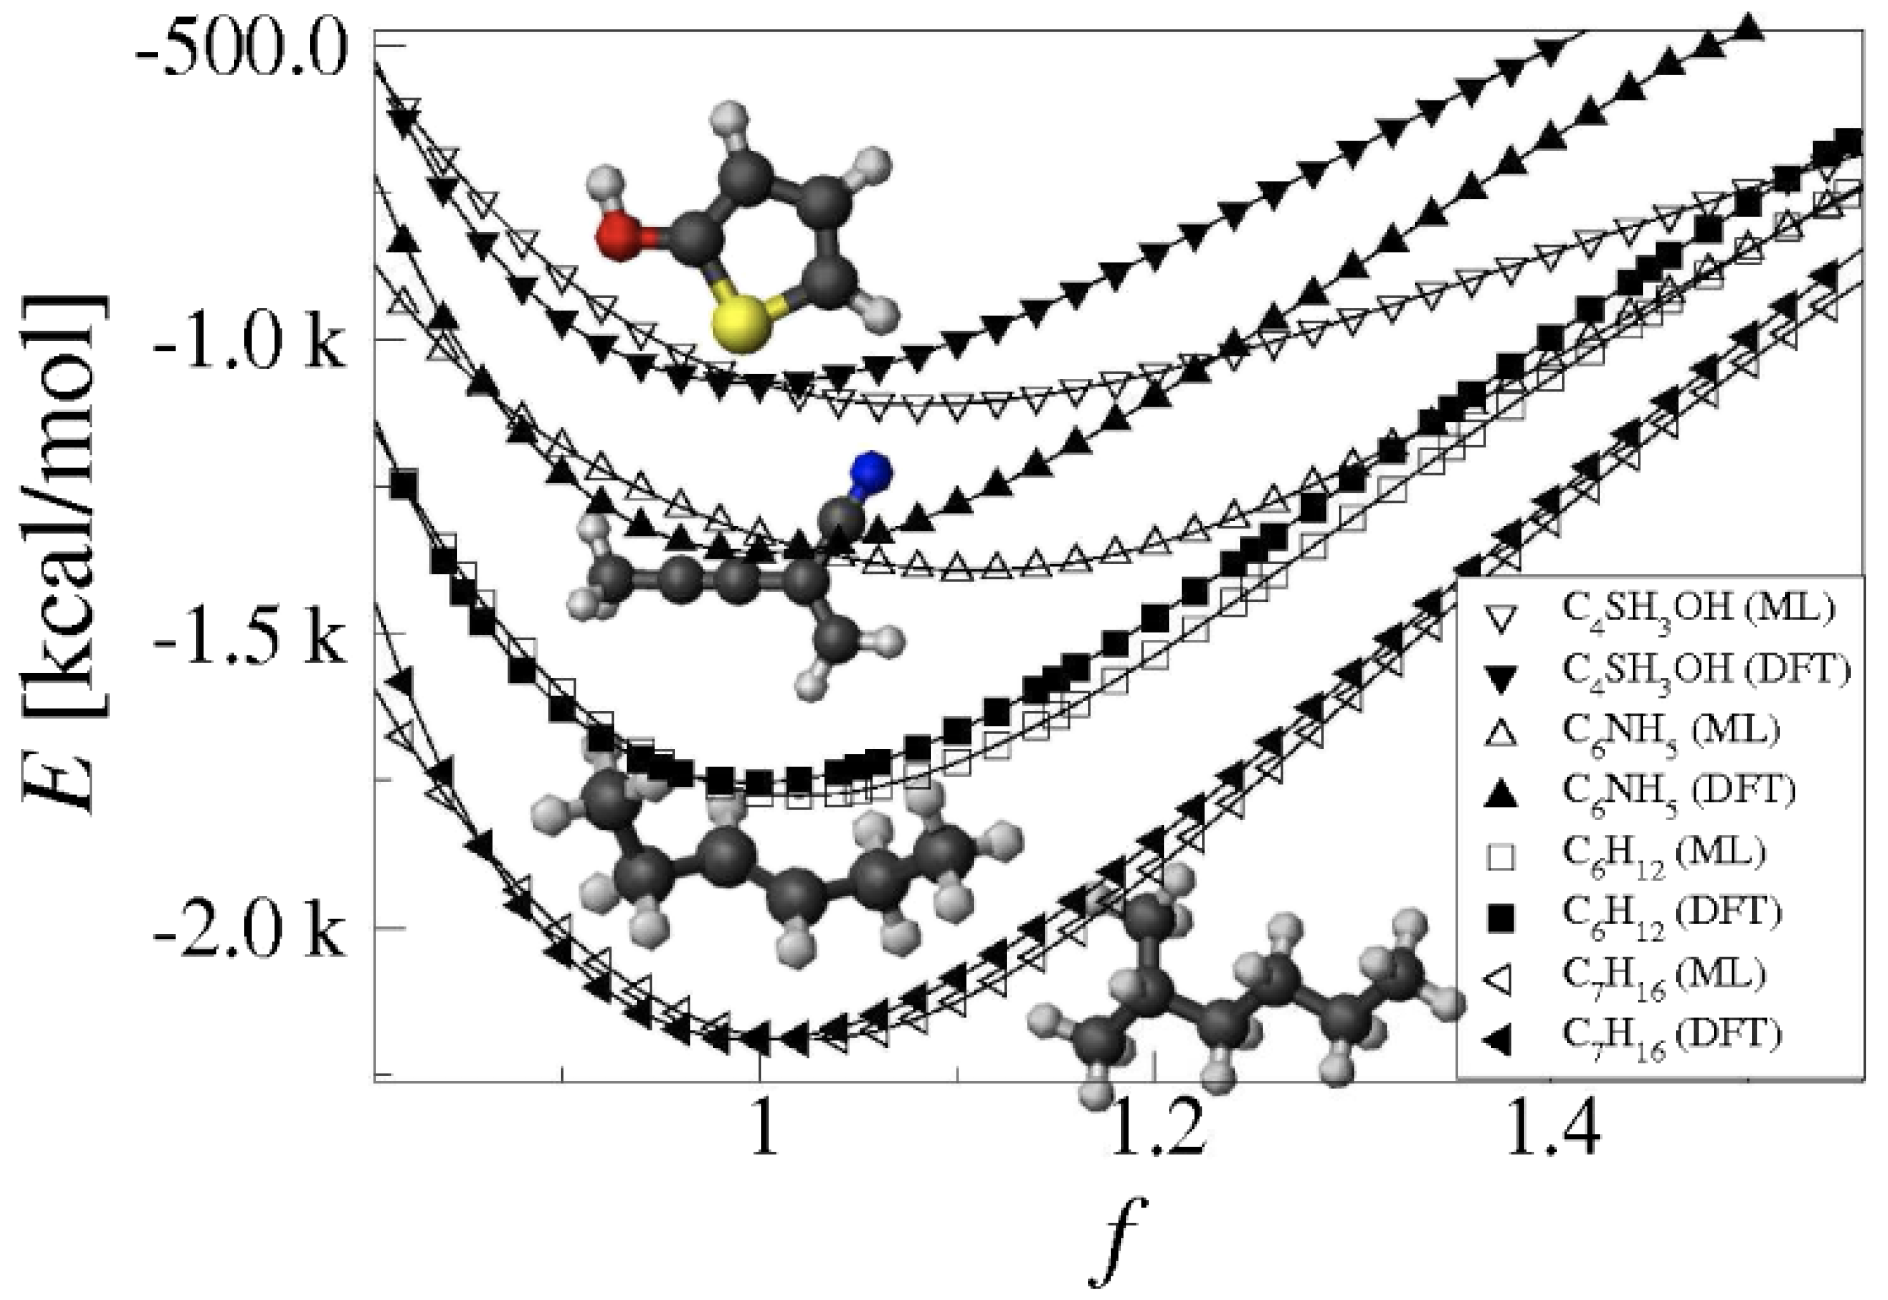
\includegraphics[width=3.5cm]{representations/images/coulomb_matrix_performance.png}};}
\visible<1->{\node[anchor=west] (figure) at (-4.5,-1.5){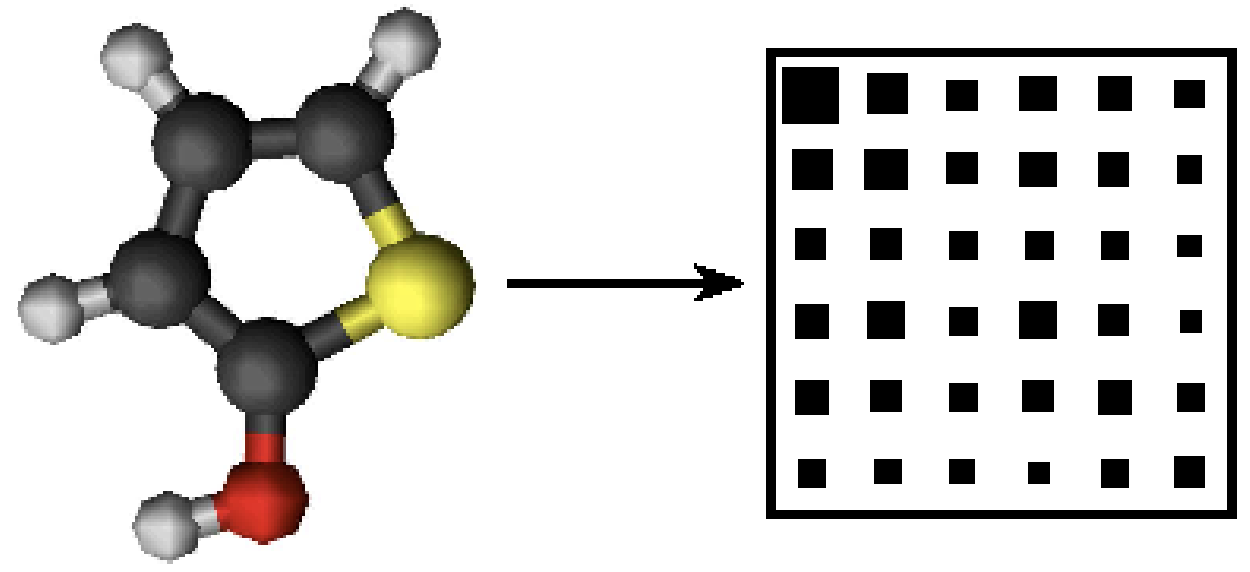
\includegraphics[width=3.5cm]{representations/images/coulomb_matrix.png}};}
\only<2->{\node[anchor = south] (text) at (1.5,-3.25){\begin{minipage}{10.0cm}
rotational and translational invariance
\end{minipage}};}
\end{tikzpicture}
\end{center}
